\documentclass[xcolor=dvipsnames]{beamer}
\usepackage[ngerman]{babel}
\usepackage[utf8]{inputenc}
\usepackage{tikz}
\usepackage{color}
\usepackage{multirow}
\usepackage{amsmath}
\usepackage{amssymb}
\usefonttheme[onlymath]{serif}
\usetikzlibrary{positioning,fit}
\pgfdeclarelayer{background}
\pgfsetlayers{background,main}
\usepackage{subfig}
\usepackage{tikz-3dplot}
\usepackage{pgfplots}
\usepackage{adjustbox}
\usepackage{extarrows}
\usepackage[weather]{ifsym}
\usepackage{mdframed}
\usepackage{bm}

\usetikzlibrary{shapes.geometric, arrows, angles, calc}

\setbeamercolor*{black}{fg=black, bg=black}
\beamertemplatenavigationsymbolsempty
%\setbeamertemplate{theorems}[numbered]

\usetheme{Berlin} %Dresden
\usecolortheme{dolphin}

\title{Multilevel Monte Carlo Methoden}
\author{Hendrik Kleikamp}
\date{5. Juli 2017}
\titlegraphic{
\includegraphics[width=2.5cm]{figures/logo.png}\hspace*{4.75cm}~%
	
\includegraphics[width=2.5cm]{figures/logo.png}}
\institute{Hauptseminar Wissenschaftliches Rechnen}

\AtBeginSection[]{\frame{\sectionpage}}
\defbeamertemplate{section page}{mine}[1][]{%
	\begin{centering}
		\begin{beamercolorbox}[sep=12pt,center]{part number}
			Kapitel \thesection
		\end{beamercolorbox}
		\vskip1em\par
		\begin{beamercolorbox}[sep=12pt,center]{part title}
			\usebeamerfont{section title}\insertsection\par
		\end{beamercolorbox}
	\end{centering}
}
\setbeamertemplate{section page}[mine]

\setlength{\abovecaptionskip}{0pt}
\setlength{\belowcaptionskip}{0pt}
\renewcommand{\footnotesize}{\fontsize{6pt}{9pt}\selectfont}


\begin{document}

\begingroup
\setbeamertemplate{headline}{}
\begin{frame}
	\titlepage
\end{frame}
\endgroup

\begin{frame}
	\frametitle{Inhaltsübersicht}
	\tableofcontents
\end{frame}

\section{Einführung}

\begin{frame}[c]
	\frametitle{Beispiel: Kurssimulationen\footnote{Weiterf. Informationen bspw. in \glqq Stochastic Differential Equations and Financial Mathematics\grqq\ von Thomas Önskog (2016, Vorlesungsunterlagen)}}
	Aktienkurse in Abhängigkeit der Zeit sind Lösungen der Stochastischen Differentialgleichung
	\[
		\mathrm{d}S(t)=a(S,t)\mathrm{d}t+b(S,t)\mathrm{d}W(t),\ \ \ \ \ 0<t<T.
	\]
	\onslide<2->{Gesucht in Anwendungen: Erwarteter Wert $\mathbb{E}[P(S)]$ des Kurses zum Zeitpunkt $T$.
	\newline
	\newline
	Wir schreiben von nun an $P$ statt $P(S)$.}
	\newline
	\newline
	\onslide<3->{\Lightning\textbf{Problem:} $\mathbb{E}[P]$ kann (oft) nicht analytisch bestimmt werden.}
\end{frame}

\begin{frame}[c]
	\frametitle{Beispiel: Kurssimulationen}
	\underline{Idee der Monte Carlo Methode:}
	\vspace{0.1cm}
	\begin{enumerate}
		\item Bestimmen (approximativ) die Lösung $S$ der SDGL.
	\onslide<2->{\item Simulieren $N$ Kursverläufe $S^{(1)},\dots,S^{(N)}$ bezüglich $S$.}
	\onslide<3->{\item Berechnen mit $P^{(i)}:=P(S^{(i)})$ den Monte Carlo Schätzer
	\begin{align}
		X:=\frac{1}{N}\sum\limits_{i=1}^N P^{(i)} \label{simpleMonteCarloKurssimulation}
	\end{align}
	als Näherung an $\mathbb{E}[P]$.}
	\end{enumerate}
	\vspace{0.5cm}
	\onslide<4->{Es ist (Erwartungstreue von $X$)
	\[
		\mathbb{E}[X]=\mathbb{E}[P]
	\]
	und
	\[
		\mathbb{V}[X]=\frac{1}{N}\mathbb{V}[P].
	\]}
\end{frame}

\begin{frame}[c]
	\frametitle{Beispiel: Kurssimulationen}
	Als root mean squared error ($RMSE$) dieses Ansatzes ergibt sich:
	\begin{eqnarray}
		RMSE&=&\sqrt{\mathbb{E}[(X-\mathbb{E}[P])^2]}\notag\\
		&=&\sqrt{\mathbb{V}[X]+(\mathbb{E}[X]-\mathbb{E}[P])^2}\notag\\
		&=&\sqrt{\frac{1}{N}\mathbb{V}[P]}\notag\\
		&=&\mathcal{O}(N^{-1/2}).\notag
	\end{eqnarray}
	\onslide<2->{Für eine Genauigkeit von $\epsilon>0$ werden also $N=\mathcal{O}(\epsilon^{-2})$ Samples benötigt.}
	\newline
	\newline
	\onslide<3->{\Lightning\textbf{Problem:} Hoher Rechenaufwand, falls $\epsilon$ klein ist.}
\end{frame}

\section{Multilevel Monte Carlo Methoden}

\begin{frame}[c]
	\frametitle{Idee der Multilevel Monte Carlo Methode}
	\textbf{Ziel:} Gleichbleibende Genauigkeit bei geringerem Rechenaufwand.
	\newline
	\newline
	\underline{Im Allgemeinen:}
	\newline
	\noindent\hspace*{5mm}Gegeben: Wahrscheinlichkeitsraum $(\Omega,\mathcal{A},\mathbb{P})$, \newline
	\noindent\hspace*{21mm}(reelle) Zufallsvariable $P$
	\newline
	\noindent\hspace*{5mm}Gesucht: $\mathbb{E}[P]$
	\newline
	\newline
	\onslide<2->{\textbf{Ansatz:} Approximieren $P$ durch eine Folge $\{P_l\}_{l\in\mathbb{N}}$ für die gilt:
	\begin{tabular}[h]{p{0.01\linewidth}p{0.87\linewidth}}
		\textcolor{green}{$\boldsymbol{\oplus}$} & Approximationsfehler von $P_l$ sinkt mit wachsendem $l$.\\
		\textcolor{red}{$\boldsymbol{\ominus}$} & Rechenaufwand für Simulationen steigt mit wachsendem $l$ monoton.
	\end{tabular}
	}
	\newline
	\newline
	\onslide<3->{\textbf{Idee:} Vorteile von kleinen und großen Leveln $l$ kombinieren, um $\mathbb{E}[P_L]$ für ein $L$ als Näherung an $\mathbb{E}[P]$ zu berechnen.}
\end{frame}

%\begin{frame}[c]
%	\frametitle{Beispiel: Kurssimulationen}
%	Unterschiedliche Diskretisierungsweiten in unterschiedlichen Leveln ($M=2^l$ Simulationspunkte in Level $l$):
%	\begin{center}
%		\begin{figure}
%			\centering
%			\subfloat[$M=4$ \label{pic:asset_prices_2}]{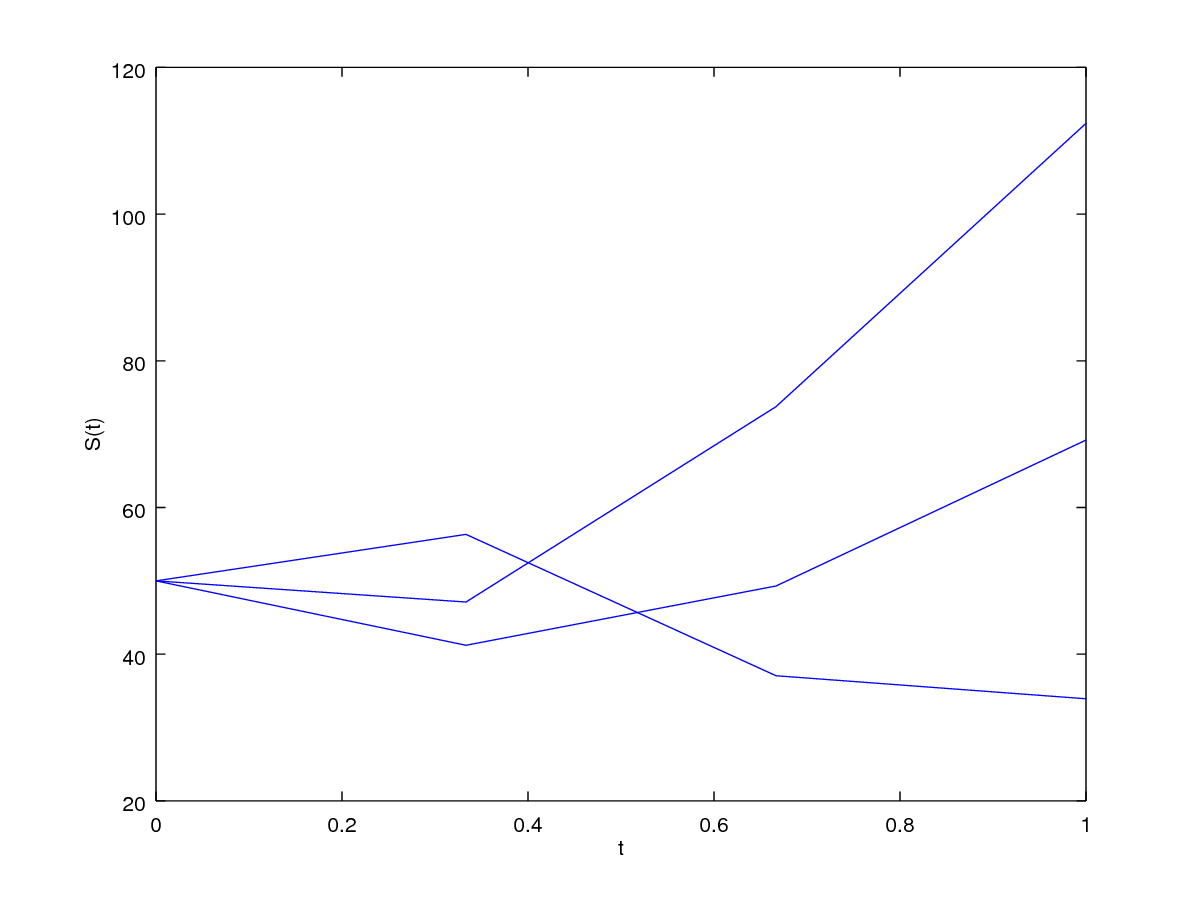
\includegraphics[width=0.45\linewidth]{figures/asset_prices_2.png}}
%			\hfill % alternativ auch \hspace{1cm} für genaue Angaben
%			\subfloat[$M=8$ \label{pic:asset_prices_3}]{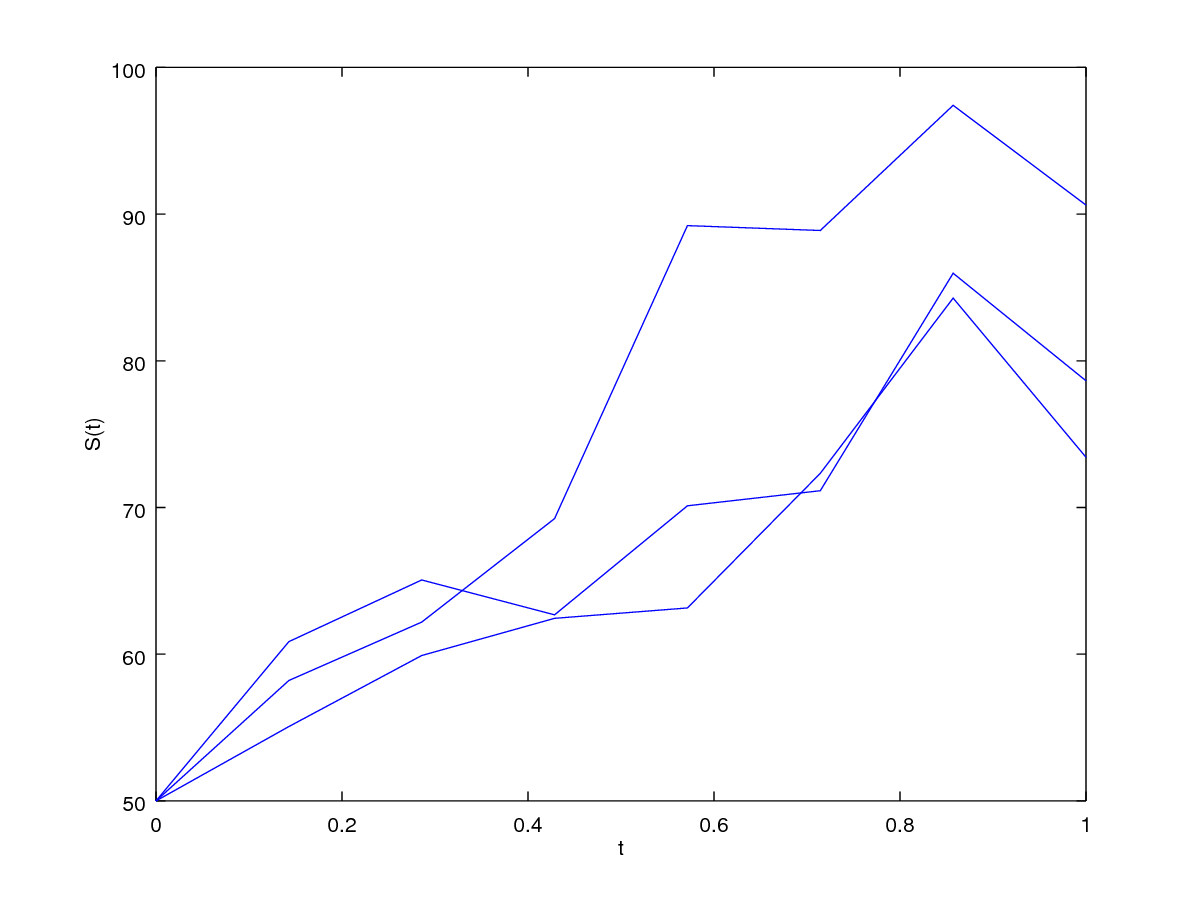
\includegraphics[width=0.45\linewidth]{figures/asset_prices_3.png}}
%		\end{figure}
%	\end{center}
%\end{frame}
%
%\begin{frame}[c]
%	\frametitle{Beispiel: Kurssimulationen}
%	Unterschiedliche Diskretisierungsweiten in unterschiedlichen Leveln ($M=2^l$ Simulationspunkte in Level $l$):
%	\begin{center}
%		\begin{figure}
%			\centering
%			\subfloat[$M=16$ \label{pic:asset_prices_4}]{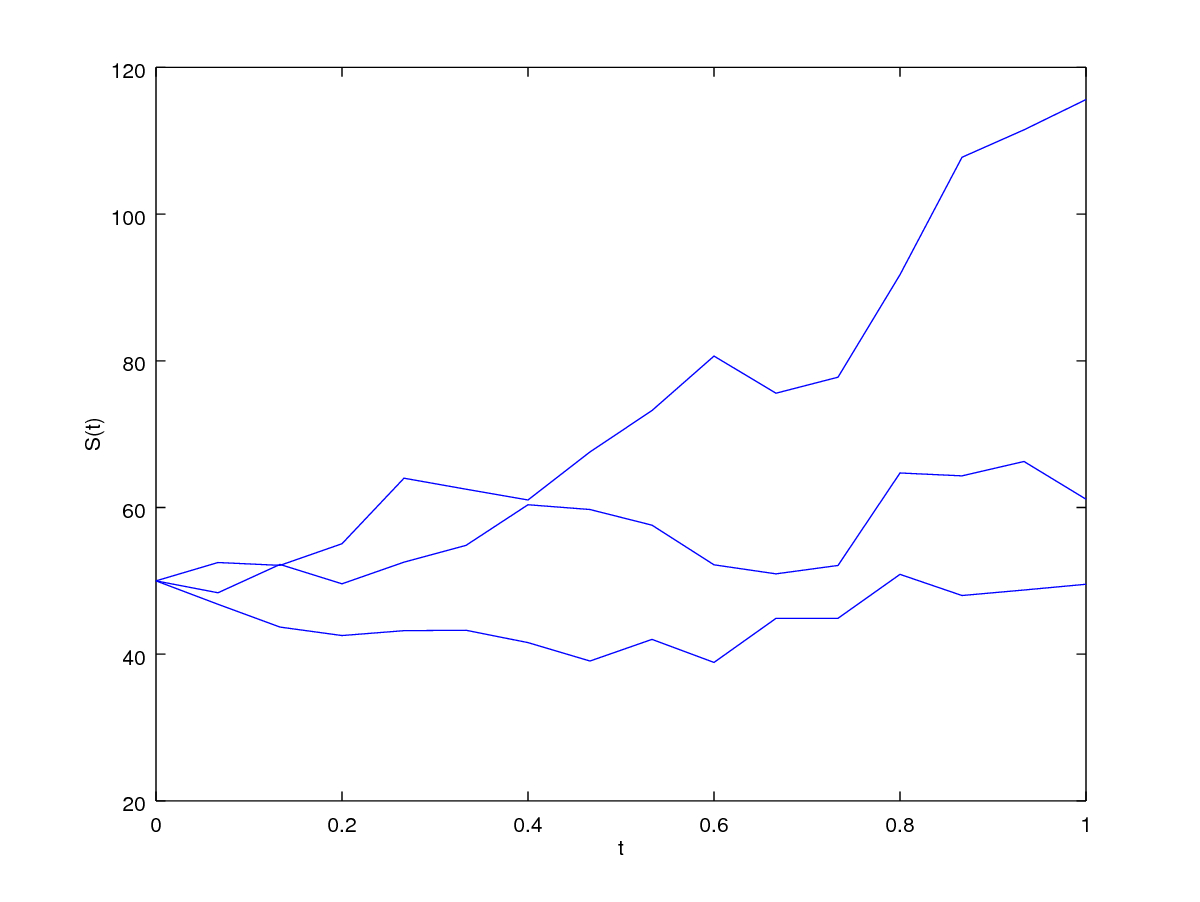
\includegraphics[width=0.45\linewidth]{figures/asset_prices_4.png}}
%			\hfill % alternativ auch \hspace{1cm} für genaue Angaben
%			\subfloat[$M=32$ \label{pic:asset_prices_5}]{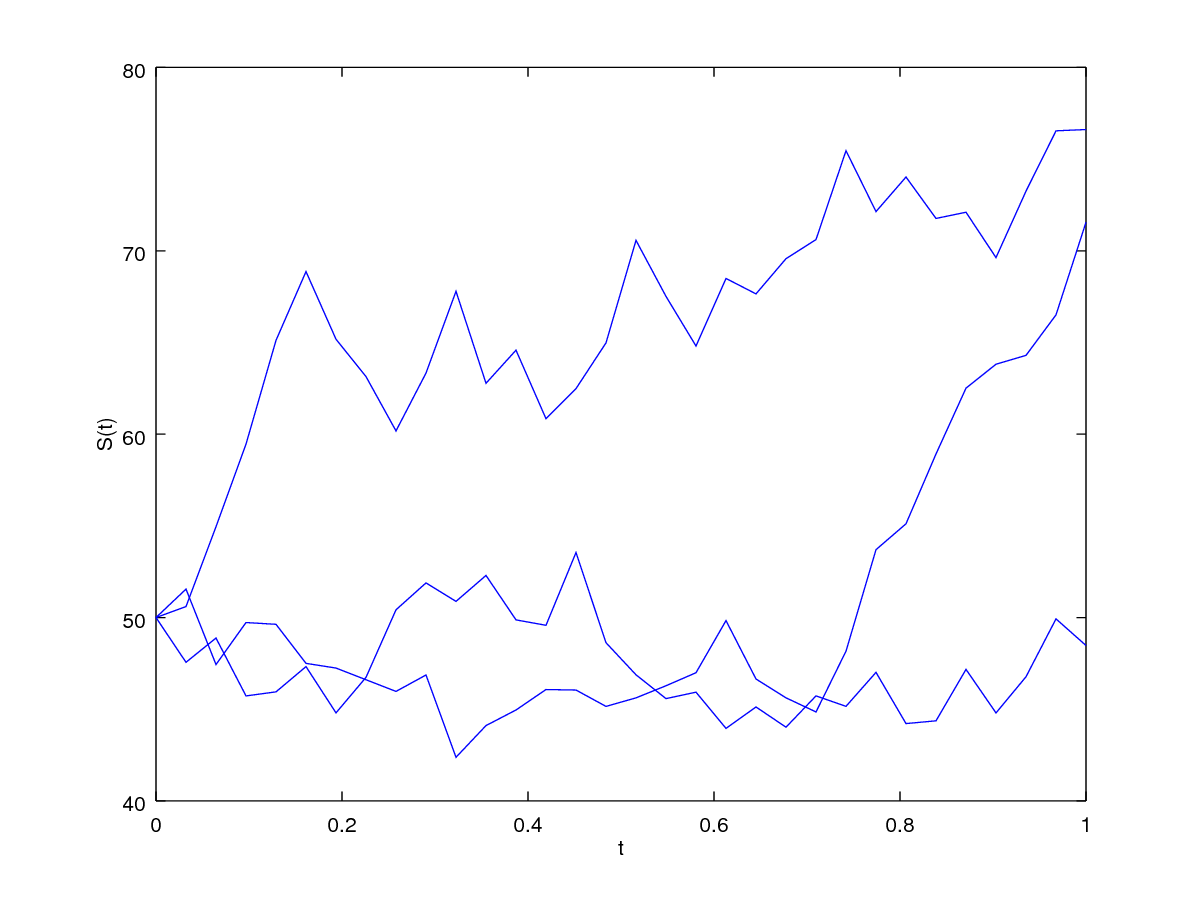
\includegraphics[width=0.45\linewidth]{figures/asset_prices_5.png}}
%		\end{figure}
%	\end{center}
%\end{frame}

\begin{frame}[c]
	\frametitle{Idee der Multilevel Monte Carlo Methode}
	Wir nutzen folgende Teleskopsumme:
	\begin{align}
		\mathbb{E}[P_L]=\mathbb{E}[P_0]+\sum\limits_{l=1}^L \mathbb{E}[P_l-P_{l-1}]. \label{teleskopsummeMultilevelMonteCarloKurssimulation}
	\end{align}
	\onslide<2->{Einsetzen eines Schätzers wie in Formel \eqref{simpleMonteCarloKurssimulation} für jeden Erwartungswert ergibt den Schätzer $Y$,
	\begin{align}
		Y:=\frac{1}{N_0}\sum\limits_{i=1}^{N_0}P_0^{(0,i)}+\sum\limits_{l=1}^L\left(\frac{1}{N_l}\sum\limits_{i=1}^{N_l}P_l^{(l,i)}-P_{l-1}^{(l,i)}\right), \label{teleskopsummeMultilevelMonteCarloKurssimulationMitSchaetzer}
	\end{align}
	für $\mathbb{E}[P_L]\approx\mathbb{E}[P]$.
	}
\end{frame}

\begin{frame}
	\frametitle{Fehler der Multilevel Monte Carlo Methode}
	Es gilt 
	\[
		\mathbb{E}[Y]=\mathbb{E}[P_L]
	\]
	und
	\[
		\mathbb{V}[Y]=\sum\limits_{l=0}^{L}\frac{1}{N_l}\mathbb{V}[P_l-P_{l-1}]
	\]
	wobei $P_{-1}\equiv 0$ gesetzt wird.
	\newline
	\onslide<2->{Dies ergibt einen mean squared error ($MSE$) von
	\begin{eqnarray}
		MSE&=&\mathbb{E}\left[(Y-\mathbb{E}[P])^2\right]\notag\\
		&=&\mathbb{V}[Y]+(\mathbb{E}[Y]-\mathbb{E}[P])^2\notag\\
		&=&\underbrace{\sum\limits_{l=0}^{L}\frac{1}{N_l}\mathbb{V}[P_l-P_{l-1}]}_{\substack{\text{Stichproben-Fehler}}}\ +\underbrace{(\mathbb{E}[P_L-P])^2}_{\substack{\text{Approximationsfehler}}}. \label{MSEMultilevelMonteCarlo}
	\end{eqnarray}}
\end{frame}

\begin{frame}[c]
	\frametitle{Konkreter: Zwei-Level Monte Carlo Methode}
	Zwei-Level Schätzer:
	\[
	Y:=\frac{1}{N_0}\sum\limits_{i=1}^{N_0}P_0^{(0,i)}+\frac{1}{N_1}\sum\limits_{i=1}^{N_1}\underbrace{P_1^{(1,i)}-P_0^{(1,i)}}_{\substack{\text{Differenz von }P_1\text{ und }P_0\\ \text{bei gleichen Samples}}}
	\]
	\newline
	\newline
	\onslide<2->{\textbf{Fragen:}
	\begin{itemize}
		\item Wie verhalten sich Berechnungskosten und Varianz des Schätzers?
		\newline
		\item Wie sollten $N_0$ und $N_1$ am besten gewählt werden?
	\end{itemize}}
\end{frame}

\begin{frame}[c]
	\frametitle{Berechnungskosten und Varianz des Zwei-Level-Schätzers}
	Seien $C_0$ und $C_1$ die Berechnungskosten für ein Sample von $P_0$ und $P_1-P_0$.
	\newline
	\underline{Gesamtkosten:} $C=N_0 C_0+N_1 C_1$
	\newline
	\newline
	\onslide<2->{Seien $V_0$ und $V_1$ die Varianzen von $P_0$ und $P_1-P_0$.
	\newline
	\underline{Varianz des Schätzers:} $V=\frac{V_0}{N_0}+\frac{V_1}{N_1}$}
	\newline
	\newline
	\onslide<3->{Sei $C$ fest. Wir minimieren $V$, wobei $N_0,N_1$ reelle Variablen seien.
	\newline
	\newline
	$\Rightarrow$ \textbf{Lagrange-Multiplikatoren-Methode}}
\end{frame}

\begin{frame}[c]
	\frametitle{Lagrange-Multiplikatoren-Methode}
	Lagrange-Funktion:
	\[
		\mathcal{L}((N_0,N_1),\mu)=\frac{V_0}{N_0}+\frac{V_1}{N_1}+\mu\cdot(N_0 C_0+N_1 C_1-C)
	\]
	\newline
	\onslide<2->{Karush-Kuhn-Tucker-Bedingungen:
	\begin{eqnarray}
	&&0\stackrel{!}{=}\nabla_{(N_0,N_1)}\mathcal{L}=\begin{bmatrix}
		-V_0/N_0^2+\mu C_0\\-V_1/N_1^2+\mu C_1
		\end{bmatrix} \notag \\
	&\Leftrightarrow&N_0=\sqrt{\frac{V_0}{\mu C_0}}\ \ \wedge\ \ N_1=\sqrt{\frac{V_1}{\mu C_1}}\label{N0N1Lagrange}
	\end{eqnarray}}
\end{frame}

\begin{frame}[c]
	\frametitle{Varianz}
	\textbf{Ziel:} Gesamtvarianz $V=\epsilon^2/2$
	\newline
	\newline
	Mit Gleichung \eqref{N0N1Lagrange} folgt:
	\begin{eqnarray}
		&&\epsilon^2/2=V\notag\\
		&\Leftrightarrow&\epsilon^2/2=V_0/N_0+V_1/N_1\notag\\
		&\Leftrightarrow&\epsilon^2/2=\sqrt{\mu V_0C_0}+\sqrt{\mu V_1C_1}\notag\\
		&\Leftrightarrow&\epsilon^2/2=\sqrt{\mu}(\sqrt{V_0C_0}+\sqrt{V_1C_1})\notag\\
		&\Leftrightarrow&\sqrt{\mu}=\frac{\epsilon^2}{2(\sqrt{V_0C_0}+\sqrt{V_1C_1})} \label{sqrtMuLagrange}
	\end{eqnarray}
\end{frame}

\begin{frame}[c]
	\frametitle{Rechenaufwand}
	Mit \eqref{N0N1Lagrange} und \eqref{sqrtMuLagrange} gilt für den Rechenaufwand $C$ nun:
	\begin{eqnarray}
		C&=&N_0C_0+N_1C_1\notag\\
		&=&\sqrt{\frac{V_0}{\mu C_0}}\ C_0+\sqrt{\frac{V_1}{\mu C_1}}\ C_1\notag\\
		&=&\frac{1}{\sqrt{\mu}}(\sqrt{V_0C_0}+\sqrt{V_1C_1})\notag\\
		&=&2\ \frac{(\sqrt{V_0C_0}+\sqrt{V_1C_1})^2}{\epsilon^2}
	\end{eqnarray}
\end{frame}

\begin{frame}[c]
	\frametitle{Optimale Anzahl von Samples}
	Zusammenfassend ergibt sich:
	\[
		N_0=\frac{1}{\sqrt{\mu}}\sqrt{\frac{V_0}{C_0}}=2\left(\frac{\sqrt{V_0C_0}+\sqrt{V_1C_1}}{\epsilon^2}\right)\sqrt{\frac{V_0}{C_0}}
	\]
	\[
		N_1=\frac{1}{\sqrt{\mu}}\sqrt{\frac{V_1}{C_1}}=2\left(\frac{\sqrt{V_0C_0}+\sqrt{V_1C_1}}{\epsilon^2}\right)\sqrt{\frac{V_1}{C_1}}
	\]
	\newline
	\newline
	\newline
	$\rightsquigarrow$ Alle Resultate lassen sich analog auf $L>1$ übertragen.
\end{frame}

\section{Hauptresultat}

\begin{frame}
	\frametitle{Multilevel Monte Carlo Theorem}
	\begin{tabular}{@{\hspace{0em}}l@{}p{8cm}}
		\textbf{Wichtig:\ } & Die Multilevel Monte Carlo Methode benötigt im Allgemeinen \underline{keine} geometrische Level-Sequenz!
	\end{tabular}
	\newline
	\newline
	\textbf{Grundlagen für das Theorem:}	
	\begin{enumerate}
		\item Geometrische Level-Sequenz
		\item Kosten wachsen exponentiell mit dem Level
		\item Fehler $|\mathbb{E}[P_l-P]|$ und Varianz $\mathbb{V}[P_l-P_{l-1}]$ sinken exponentiell mit dem Level
	\end{enumerate}
	\textbf{Ziele:}
	\begin{enumerate}
		\item $\mathbb{V}[Y]<\epsilon^2/2$
		\item $(\mathbb{E}[P_L-P])^2<\epsilon^2/2$
	\end{enumerate}
	\hspace{0.275cm}$\xLongrightarrow{\eqref{MSEMultilevelMonteCarlo}} MSE<\epsilon^2$
\end{frame}

\begin{frame}
	\begin{theorem}[MLMC $\lbrack$Giles, 2015$\rbrack$]
		Sei $P$ eine Zufallsvariable und $P_l$ eine numerische Approximation an $P$ im Level $l$. 
		\newline
		Angenommen, es existieren unabhängige Schätzer $Y_l$ basierend auf $N_l$ Monte Carlo Samples, jeweils mit erwarteten Kosten $C_l$ und einer Varianz $V_l$, sowie positive Konstanten $\alpha,\beta,\gamma,c_1,c_2,c_3$ mit $\alpha\geq\frac{1}{2}\min(\beta,\gamma)$ und
		\begin{enumerate}
			\item $|\mathbb{E}[P_l-P]|\leq c_1 2^{-\alpha l}$
			\item $\mathbb{E}[Y_l]=\begin{cases}\mathbb{E}[P_0], & l=0 \\ \mathbb{E}[P_l-P_{l-1}], & l>0\end{cases}$
			\item $V_l\leq c_2 2^{-\beta l}$
			\item $C_l\leq c_3 2^{\gamma l}$.
		\end{enumerate}
	\end{theorem}
\end{frame}

\begin{frame}
	\begin{theorem}[MLMC $\lbrack$Giles, 2015$\rbrack$]
		Dann gibt es eine Konstante $c_4>0$, sodass für alle $\epsilon<e^{-1}$ Zahlen $L$ und $N_l$ existieren, für die der Multilevel-Schätzer
		\[
			Y:=\sum\limits_{l=0}^L Y_l
		\]
		einen Fehler von
		\[
			MSE=\mathbb{E}\left[(Y-\mathbb{E}[P])^2\right]<\epsilon^2
		\]
		besitzt und der Rechenaufwand $C$ insgesamt beschränkt ist durch
		\[
			\mathbb{E}[C]\leq\begin{cases}c_4\epsilon^{-2}, & \beta>\gamma \\ c_4\epsilon^{-2}(\log\epsilon)^2, & \beta=\gamma \\ c_4\epsilon^{-2-(\gamma-\beta)/\alpha}, & \beta<\gamma.\end{cases}
		\]
	\end{theorem}
\end{frame}

\begin{frame}[c]
	\frametitle{Hinweise zum MLMC-Theorem I\footnote{Ein Beweis des Theorems findet sich in \glqq Multilevel Monte Carlo methods and applications to elliptic PDEs with random coefficients\grqq\ von Cliffe et al. (2011)}}
	Wofür werden die vielen Annahmen benötigt?
	\newline
	\newline
	Bedingung....
	\begin{enumerate}
		\item sichert, dass $|\mathbb{E}[P_l-P]|\xlongrightarrow{l\to\infty}0$,
		\item sichert, dass $\mathbb{E}[Y]=\mathbb{E}[P_L]$,
		\item sichert, dass $V_l\xlongrightarrow{l\to\infty}0$,
		\item sichert, dass $C_l<\infty\ \ \forall\ l\geq 0$.
	\end{enumerate}
\end{frame}

\begin{frame}[c]
	\frametitle{Hinweise zum MLMC-Theorem II}
	\begin{mdframed}[innertopmargin=-15pt,innerbottommargin=5pt,linewidth=0.5pt,topline=true,roundcorner=5pt,innerleftmargin=5pt,backgroundcolor=yellow!20,linecolor=yellow,frametitle={Erinnerung:}]
	\[
		C=2\ \frac{\left(\sum\limits_{l=0}^L\sqrt{V_lC_l}\right)^2}{\epsilon^2}\stackrel{Ann.3+4}{\leq}2\ \frac{\left(\sum\limits_{l=0}^L c_2c_3 2^{l(\gamma-\beta)/2}\right)^2}{\epsilon^2}
	\]
	\end{mdframed}
	\vspace{0.3cm}
	\onslide<2->{Fall 1: $\beta>\gamma$
	\newline
	\noindent\hspace*{6mm}$\rightarrow$ Größter Rechenaufwand im gröbsten Level
	}
	\newline
	\newline
	\onslide<3->{Fall 2: $\beta<\gamma$
	\newline
	\noindent\hspace*{6mm}$\rightarrow$ Größter Rechenaufwand im feinsten Level
	}
	\newline
	\newline
	\onslide<4->{Fall 3: $\beta=\gamma$
	\newline
	\noindent\hspace*{6mm}$\rightarrow$ Rechenaufwand in jedem Level ungefähr gleich (Produkt \noindent\hspace*{11mm}aus Varianz und Kosten unabhängig vom Level)}
\end{frame}

\begin{frame}[c]
	\frametitle{Hinweise zum MLMC-Theorem III}
	\begin{itemize}
		\item Schätzer $Y_l$ kann beliebig konstruiert werden, solange die Voraussetzungen des MLMC-Theorems erfüllt sind
		\newline
		\item Aufteilung des Fehlers $\epsilon^2$ gleichermaßen auf $(\mathbb{E}[P_L-P])^2$ und $\mathbb{V}[Y]$ ist nicht immer optimal
	\end{itemize}
\end{frame}

\section{Implementierung}

\begin{frame}
	\frametitle{Der Algorithmus}
	
	\tikzstyle{startstop} = [rectangle, rounded corners, minimum width=3cm, minimum height=1cm, text centered, draw=red, fill=red!30]
	\tikzstyle{process} = [rectangle, minimum width=3cm, minimum height=1cm, text centered, text width=3cm, draw=orange, fill=orange!30]
	\tikzstyle{decision} = [diamond, minimum width=3cm, minimum height=1cm, text centered, draw=green, fill=green!30, aspect=3]
	\tikzstyle{arrow} = [thick,->,>=stealth]
	
	\begin{tikzpicture}[node distance=1.75cm]
	
	\node (initialisieren) [process] {Initialisieren};
	
	\onslide<2->{
	\node (weitereSamples) [decision, below of=initialisieren] {Mehr Samples?};
	}
	
	\onslide<3->{
	\node (stop) [startstop, right of=weitereSamples, xshift=4cm] {Stop};
	
	\node (samplesAuswerten) [process, below of=weitereSamples, yshift=-0.75cm] {Weitere Samples auswerten,\\$V_l$ schätzen,\\optimales $N_l$ berechnen};
	}
	
	\onslide<4->{
	\node (konvergenz) [decision, right of=samplesAuswerten, xshift=4cm] {Konvergenz?};
	}
	
	\onslide<5->{
	\node (LPlusEins) [process, below of=konvergenz] {Setze $L:=L+1$,\\initialisiere $N_L$};
	}
	
	\onslide<2->{
	\draw [arrow] (initialisieren) -- (weitereSamples);
	}
	\onslide<3->{
	\draw [arrow] (weitereSamples) -- node[anchor=south] {nein} (stop);
	\draw [arrow] (weitereSamples) -- node[anchor=east] {ja} (samplesAuswerten);
	}
	\onslide<4->{
	\draw [arrow] (samplesAuswerten) -- (konvergenz);
	}
	\onslide<5->{
	\draw [arrow] (konvergenz) -- node[anchor=east] {nein} (LPlusEins);
	\draw [arrow] (konvergenz) -- node[anchor=east] {ja} (stop);
	\draw [arrow] (LPlusEins) -- (-3,-6) -- (-3,-1.75) -- (weitereSamples);
	}

	\end{tikzpicture}
\end{frame}

\begin{frame}[c]
	\frametitle{Hinweise zur Implementierung}
	\begin{itemize}
		\item Die Konstanten $c_1$ und $c_2$ sind meist nicht bekannt.
		\item Die Genauigkeit der Schätzer für $V_l$ $(l=0,\dots,L)$ hängt von der Anzahl der verwendeten Samples ab.
		\newline
		\newline
		\item \textbf{Wichtig:} Der Algorithmus ist heuristisch, ein $MSE$ von $\epsilon^2$ ist \noindent\hspace*{16.25mm}nicht garantiert!
	\end{itemize}
\end{frame}

\begin{frame}[c]
	\frametitle{Besonderheiten bei der Implementierung\footnote{Für eine konkrete Umsetzung des MLMC-Algorithmus mit sämtlichen Besonderheiten siehe \cite{giles2015} und http://people.maths.ox.ac.uk/gilesm/mlmc/ (C/C++ und MATLAB-Code)}}
	\begin{itemize}
		\item Der Konvergenz-Test überprüft, ob $|\mathbb{E}[P_L-P]|<\epsilon/\sqrt{2}$ um den gewünschten $MSE$ zu erhalten:
		\[
			\left|\mathbb{E}[P-P_L]\right|=\left|\sum\limits_{l=L+1}^{\infty}\mathbb{E}[P_l-P_{l-1}]\right|=\left|\frac{\mathbb{E}[P_L-P_{L-1}]}{(2^\alpha-1)}\right|\stackrel{!}{<}\epsilon/\sqrt{2}
		\]
		\item Sind $\alpha$ und $\beta$ nicht bekannt, so müssen diese, bspw. mittels linearer Regression, geschätzt werden.
	\end{itemize}
\end{frame}

\section{Multi-Index Monte Carlo}

\begin{frame}
	\frametitle{Erweiterung: Multi-Index Monte Carlo\footnote{Weiterf. Informationen in \glqq Multi index Monte Carlo: when sparsity meets sampling\grqq\ von Haji-Ali et al. (2014)}}
	\textbf{Idee:} Mehrdimensionale Levelindizes
	\newline
	$\Rightarrow$ Ermöglicht bspw. unterschiedliche Diskretisierungsweiten in \noindent\hspace*{5mm}unterschiedliche Koordinatenrichtungen.
	\begin{figure}[H]
		\centering
		\begin{adjustbox}{width=0.4\paperwidth, center}
			\begin{tikzpicture}
				\begin{axis} [ 
					style=thick, 
					xlabel=$l_1$,
					ylabel=$l_2$,
					minor tick num=0, 
					xmin=0, xmax=5,  
					ymin=0, ymax=5,
					axis x line=middle,
					axis y line=middle,
					xtick={0,1,...,5},
					ytick={0,1,...,5}
				  ]
					\node[circle,fill,inner sep=1.5pt] (P11) at (axis cs:1,1) {};
					\node[circle,fill,inner sep=1.5pt] (P12) at (axis cs:1,2) {};
					\node[circle,fill,inner sep=1.5pt] (P21) at (axis cs:2,1) {};
					\node[circle,fill,inner sep=1.5pt] (P22) at (axis cs:2,2) {};
					\node[circle,fill,inner sep=1.5pt] (P31) at (axis cs:3,1) {};
					\node[circle,fill,inner sep=1.5pt] (P32) at (axis cs:3,2) {};
					\node[circle,fill,inner sep=1.5pt] (P33) at (axis cs:3,3) {};
					\node[circle,fill,inner sep=1.5pt] (P13) at (axis cs:1,3) {};
					\node[circle,fill,inner sep=1.5pt] (P23) at (axis cs:2,3) {};
					\node[circle,fill,inner sep=1.5pt] (P41) at (axis cs:4,1) {};
					\node[circle,fill,inner sep=1.5pt] (P42) at (axis cs:4,2) {};
					\node[circle,fill,inner sep=1.5pt] (P43) at (axis cs:4,3) {};
					\node[label={$L=(4,4)$},circle,fill,inner sep=2.5pt] (P44) at (axis cs:4,4) {};
					\node[circle,fill,inner sep=1.5pt] (P14) at (axis cs:1,4) {};
					\node[circle,fill,inner sep=1.5pt] (P24) at (axis cs:2,4) {};
					\node[circle,fill,inner sep=1.5pt] (P34) at (axis cs:3,4) {};
					\node[circle,fill,inner sep=1.5pt] (P01) at (axis cs:0,1) {};
					\node[circle,fill,inner sep=1.5pt] (P02) at (axis cs:0,2) {};
					\node[circle,fill,inner sep=1.5pt] (P03) at (axis cs:0,3) {};
					\node[circle,fill,inner sep=1.5pt] (P04) at (axis cs:0,4) {};
					\node[circle,fill,inner sep=1.5pt] (P10) at (axis cs:1,0) {};
					\node[circle,fill,inner sep=1.5pt] (P20) at (axis cs:2,0) {};
					\node[circle,fill,inner sep=1.5pt] (P30) at (axis cs:3,0) {};
					\node[circle,fill,inner sep=1.5pt] (P40) at (axis cs:4,0) {};
					\node[circle,fill,inner sep=1.5pt] (P00) at (axis cs:0,0) {};
					\draw [-] (P03) to (P43);
					\draw [-] (P30) to (P34);
					\draw [-] (P02) to (P42);
					\draw [-] (P20) to (P24);
					\draw [-] (P40) to (P44);
					\draw [-] (P04) to (P44);
					\draw [-] (P01) to (P41);
					\draw [-] (P10) to (P14);
				\end{axis} 
			\end{tikzpicture}
		\end{adjustbox}
		\caption{Zwei-dimensionale Indizes}
		\label{}
	\end{figure}
\end{frame}

\begin{frame}
	\frametitle{Multilevel Teleskopsumme im Mehrdimensionalen}
	Wir definieren für $l=(l_i)_{i=1}^d\in\mathbb{N}^d$ die Differenz
	\[
		\Delta_iP_l=\begin{cases}
		P_l-P_{l-e_i}, & l_i>0\\P_l, & l_i=0
		\end{cases}
	\]
	wobei $e_i$ den Einheitsvektor in Koordinatenrichtung $i$ bezeichnet.
	\onslide<2->{
	\newline
	Sei zudem
	\[
		\Delta P_l=\left(\prod\limits_{i=1}^d\Delta_i\right)P_l.
	\]
	}
	\onslide<3->{
	\newline
	Es ergibt sich mit $I=\{l\in\mathbb{N}^d:l\geq 0\}$ der Schätzer
	\[
		Y:=\sum\limits_{l\in I}\mathbb{E}[\Delta P_l]
	\]
	für $\mathbb{E}[P]$.
	}
\end{frame}

\begin{frame}
	\frametitle{Beispiel: Natürliche Wahl von $I$}
	Sei
	\[
		I=\left\{(l_1,l_2)\in\mathbb{N}^2:0\leq l_1\leq 3\ \text{und}\ 0\leq l_2\leq 2\right\}.
	\]
	\onslide<2->{
	$I$ entspricht nun einem Rechteck mit Eckpunkt $(3,2)$.
	\begin{figure}[H]
		\centering
		\begin{adjustbox}{width=0.35\paperwidth, center}
			\begin{tikzpicture} 
				\begin{axis} [ 
					style=thick, 
					xlabel=$l_1$,
					ylabel=$l_2$,
					minor tick num=0, 
					xmin=0, xmax=4,  
					ymin=0, ymax=3,
					axis x line=middle,
					axis y line=middle,
					xtick={0,1,...,4},
					ytick={0,1,...,3}
				  ]
					\node[circle,fill,inner sep=1.5pt] (P11) at (axis cs:1,1) {};
					\node[circle,fill,inner sep=1.5pt] (P12) at (axis cs:1,2) {};
					\node[circle,fill,inner sep=1.5pt] (P21) at (axis cs:2,1) {};
					\node[circle,fill,inner sep=1.5pt] (P22) at (axis cs:2,2) {};
					\node[circle,fill,inner sep=1.5pt] (P31) at (axis cs:3,1) {};
					\node[label={$(3,2)$},circle,fill,inner sep=2.5pt] (P32) at (axis cs:3,2) {};
					\node[circle,fill,inner sep=1.5pt] (P01) at (axis cs:0,1) {};
					\node[circle,fill,inner sep=1.5pt] (P02) at (axis cs:0,2) {};
					\node[circle,fill,inner sep=1.5pt] (P30) at (axis cs:3,0) {};
					\node[circle,fill,inner sep=1.5pt] (P10) at (axis cs:1,0) {};
					\node[circle,fill,inner sep=1.5pt] (P20) at (axis cs:2,0) {};
					\node[circle,fill,inner sep=1.5pt] (P00) at (axis cs:0,0) {};
					\draw [-] (P02) to (P32);
					\draw [-] (P30) to (P32);
					\draw [-] (P20) to (P22);
					\draw [-] (P01) to (P31);
					\draw [-] (P10) to (P12);
				\end{axis} 
			\end{tikzpicture}
		\end{adjustbox}
	\end{figure}
	Dann ist $\Delta P_{(3,2)}=\Delta_1\Delta_2 P_{(3,2)}=P_{(3,2)}-P_{(2,2)}-P_{(3,1)}+P_{(2,1)}$ und $Y=\mathbb{E}[P_{(3,2)}]$.
	}
\end{frame}

\begin{frame}[t]
	\frametitle{Wie sollte $I$ gewählt werden?}
	Die optimale Wahl ist (ähnlich zu dünnen Gittern)
	\[
		I=\{l\in\mathbb{N}^d:l\geq 0,\ \langle l,n\rangle\leq L\}
	\]
	für eine Richtung $n\in\mathbb{N}^d,n>0,$ und ein $L\in\mathbb{N}$.
	\begin{figure}[H]
		\only<2->{
		\centering
		\begin{adjustbox}{height=0.46\paperheight, center}
			\begin{tikzpicture} 
				\begin{axis} [ 
					style=thick,
					xlabel=$l_1$,
					ylabel=$l_2$,
					minor tick num=0,
					xmin=0, xmax=7,
					ymin=1, ymax=4,
					axis x line=middle,
					axis y line=middle,
					xtick={0,1,...,7},
					ytick={0,1,...,4},
					axis equal
				  ]
					\node[circle,fill,inner sep=1.5pt] (P11) at (axis cs:1,1) {};
					\node[circle,fill,inner sep=1.5pt] (P12) at (axis cs:1,2) {};
					\node[circle,fill,inner sep=1.5pt] (P21) at (axis cs:2,1) {};
					\node[circle,fill,inner sep=1.5pt] (P22) at (axis cs:2,2) {};
					\node[circle,fill,inner sep=1.5pt] (P31) at (axis cs:3,1) {};
					\node[circle,fill,inner sep=1.5pt] (P01) at (axis cs:0,1) {};
					\node[circle,fill,inner sep=1.5pt] (P02) at (axis cs:0,2) {};
					\node[circle,fill,inner sep=1.5pt] (P03) at (axis cs:0,3) {};
					\node[circle,fill,inner sep=1.5pt] (P10) at (axis cs:1,0) {};
					\node[circle,fill,inner sep=1.5pt] (P20) at (axis cs:2,0) {};
					\node[circle,fill,inner sep=1.5pt] (P30) at (axis cs:3,0) {};
					\node[circle,fill,inner sep=1.5pt] (P40) at (axis cs:4,0) {};
					\node[circle,fill,inner sep=1.5pt] (P50) at (axis cs:5,0) {};
					\node[circle,fill,inner sep=1.5pt] (P60) at (axis cs:6,0) {};
					\node[circle,fill,inner sep=1.5pt] (P41) at (axis cs:4,1) {};
					\node[circle,fill,inner sep=1.5pt] (P00) at (axis cs:0,0) {};
					\draw [-] (P60) to (P03);
					\draw [-] (P30) to (P31);
					\draw [-] (P20) to (P22);
					\draw [-] (P02) to (P22);
					\draw [-] (P01) to (P41);
					\draw [-] (P10) to (P12);
					\draw [-] (P40) to (P41);
					\draw [-] (P50) to (axis cs:5,0.5);
					\draw [-] (P31) to (axis cs:3,1.5);
					\draw [-] (P12) to (axis cs:1,2.5);
					\only<3->{
						\node (N) at (axis cs:4,3.5) {};
						\draw [->,color=red, line width=1pt] (axis cs:3,1.5) to (N) node [below right] {$\bm{n}$};
						\node (TEMP) at (axis cs:3,1.5) {};
						\pic[draw=black,angle eccentricity=0.5,angle radius=.5cm, color=red, line width=1pt, pic text={$\bm{\cdot}$}]
						{angle=N--TEMP--P22};
					}
				\end{axis} 
			\end{tikzpicture}
		\end{adjustbox}
		\caption{Beispiel mit $L=6$ und $n=[1,2]^T$}
	}
	\end{figure}

	
%	\begin{figure}[H]
%		\centering
%		\begin{adjustbox}{width=0.4\paperwidth, center}
%			\begin{tikzpicture} 
%				\begin{axis} [ 
%					style=thick, 
%					xlabel=$l_1$,
%					ylabel=$l_2$,
%					minor tick num=0, 
%					xmin=0, xmax=5,  
%					ymin=0, ymax=5,
%					axis x line=middle,
%					axis y line=middle,
%					xtick={0,1,...,5},
%					ytick={0,1,...,5}
%				  ]
%					\node[circle,fill,inner sep=1.5pt] (P11) at (axis cs:1,1) {};
%					\node[circle,fill,inner sep=1.5pt] (P12) at (axis cs:1,2) {};
%					\node[circle,fill,inner sep=1.5pt] (P21) at (axis cs:2,1) {};
%					\node[circle,fill,inner sep=1.5pt] (P22) at (axis cs:2,2) {};
%					\node[circle,fill,inner sep=1.5pt] (P31) at (axis cs:3,1) {};
%					\node[circle,fill,inner sep=1.5pt] (P13) at (axis cs:1,3) {};
%					\node[circle,fill,inner sep=1.5pt] (P01) at (axis cs:0,1) {};
%					\node[circle,fill,inner sep=1.5pt] (P02) at (axis cs:0,2) {};
%					\node[circle,fill,inner sep=1.5pt] (P03) at (axis cs:0,3) {};
%					\node[circle,fill,inner sep=1.5pt] (P04) at (axis cs:0,4) {};
%					\node[circle,fill,inner sep=1.5pt] (P10) at (axis cs:1,0) {};
%					\node[circle,fill,inner sep=1.5pt] (P20) at (axis cs:2,0) {};
%					\node[circle,fill,inner sep=1.5pt] (P30) at (axis cs:3,0) {};
%					\node[circle,fill,inner sep=1.5pt] (P40) at (axis cs:4,0) {};
%					\node[circle,fill,inner sep=1.5pt] (P00) at (axis cs:0,0) {};
%					\draw [-] (P40) to (P04);
%					\draw [-] (P03) to (P13);
%					\draw [-] (P30) to (P31);
%					\draw [-] (P20) to (P22);
%					\draw [-] (P02) to (P22);
%					\draw [-] (P01) to (P31);
%					\draw [-] (P10) to (P13);
%				\end{axis} 
%			\end{tikzpicture}
%		\end{adjustbox}
%		\caption{Beispiel für $L=4$ und $n=[1,1]^T$}
%		\label{}
%	\end{figure}
\end{frame}

\begin{frame}[c]
	\frametitle{Optimale Wahl von $I$ in 3D}
	\tdplotsetmaincoords{70}{110}
	\begin{figure}[H]
		\centering
		\begin{adjustbox}{width=0.49\paperwidth, center}
			\begin{tikzpicture}[tdplot_main_coords]
				\coordinate[circle,fill,inner sep=1.5pt] (P112) at (1,1,2);
				\coordinate[circle,fill,inner sep=1.5pt] (P121) at (1,2,1);
				\coordinate[circle,fill,inner sep=1.5pt] (P211) at (2,1,1);
				\coordinate[circle,fill,inner sep=1.5pt] (P111) at (1,1,1);
				\coordinate[circle,fill,inner sep=1.5pt] (P021) at (0,2,1);
				\coordinate[circle,fill,inner sep=1.5pt] (P031) at (0,3,1);
				\coordinate[circle,fill,inner sep=1.5pt] (P011) at (0,1,1);
				\coordinate[circle,fill,inner sep=1.5pt] (P012) at (0,1,2);
				\coordinate[circle,fill,inner sep=1.5pt] (P022) at (0,2,2);
				\coordinate[circle,fill,inner sep=1.5pt] (P013) at (0,1,3);
				\coordinate[circle,fill,inner sep=1.5pt] (P040) at (0,4,0);
				\coordinate[circle,fill,inner sep=1.5pt] (P004) at (0,0,4);
				\coordinate[circle,fill,inner sep=1.5pt] (P030) at (0,3,0);
				\coordinate[circle,fill,inner sep=1.5pt] (P130) at (1,3,0);
				\coordinate[circle,fill,inner sep=1.5pt] (P020) at (0,2,0);
				\coordinate[circle,fill,inner sep=1.5pt] (P120) at (1,2,0);
				\coordinate[circle,fill,inner sep=1.5pt] (P220) at (2,2,0);
				\coordinate[circle,fill,inner sep=1.5pt] (P010) at (0,1,0);
				\coordinate[circle,fill,inner sep=1.5pt] (P110) at (1,1,0);
				\coordinate[circle,fill,inner sep=1.5pt] (P210) at (2,1,0);
				\coordinate[circle,fill,inner sep=1.5pt] (P310) at (3,1,0);
				\coordinate[circle,fill,inner sep=1.5pt] (P003) at (0,0,3);
				\coordinate[circle,fill,inner sep=1.5pt] (P103) at (1,0,3);
				\coordinate[circle,fill,inner sep=1.5pt] (P002) at (0,0,2);
				\coordinate[circle,fill,inner sep=1.5pt] (P102) at (1,0,2);
				\coordinate[circle,fill,inner sep=1.5pt] (P202) at (2,0,2);
				\coordinate[circle,fill,inner sep=1.5pt] (P001) at (0,0,1);
				\coordinate[circle,fill,inner sep=1.5pt] (P101) at (1,0,1);
				\coordinate[circle,fill,inner sep=1.5pt] (P201) at (2,0,1);
				\coordinate[circle,fill,inner sep=1.5pt] (P301) at (3,0,1);
				\coordinate[circle,fill,inner sep=1.5pt] (P100) at (1,0,0);
				\coordinate[circle,fill,inner sep=1.5pt] (P200) at (2,0,0);
				\coordinate[circle,fill,inner sep=1.5pt] (P300) at (3,0,0);
				\coordinate[circle,fill,inner sep=1.5pt] (P400) at (4,0,0);
				\coordinate[circle,fill,inner sep=1.5pt] (P000) at (0,0,0);
				\draw[->] (0,0,0) -- (5,0,0) node[anchor=north east]{$l_1$};
				\draw[->] (0,0,0) -- (0,5,0) node[anchor=north west]{$l_2$};
				\draw[->] (0,0,0) -- (0,0,5) node[anchor=south]{$l_3$};

				\draw[-] (P400) -- (P040) -- (P004) -- (P400);

				\draw[-] (P100) -- (P130);
				\draw[-] (P130) -- (P030);
				\draw[-] (P200) -- (P220);
				\draw[-] (P220) -- (P020);
				\draw[-] (P300) -- (P310);
				\draw[-] (P310) -- (P010);
				\draw[-] (P101) -- (P121);
				\draw[-] (P121) -- (P021);
				\draw[-] (P201) -- (P211);
				\draw[-] (P211) -- (P011);
				\draw[-] (P001) -- (P301);
				\draw[-] (P001) -- (P031);
				\draw[-] (P301) -- (P031);
				\draw[-] (P002) -- (P202);
				\draw[-] (P002) -- (P022);
				\draw[-] (P102) -- (P112);
				\draw[-] (P112) -- (P012);
				\draw[-] (P202) -- (P022);
				\draw[-] (P103) -- (P013);
				\draw[-] (P003) -- (P103);
				\draw[-] (P003) -- (P013);
				\draw[-] (P130) -- (P030);
				\draw[-] (P100) -- (P103);
				\draw[-] (P200) -- (P202);
				\draw[-] (P130) -- (P030);
				\draw[-] (P300) -- (P301);
				\draw[-] (P110) -- (P112);
				\draw[-] (P210) -- (P211);
				\draw[-] (P120) -- (P121);
				\draw[-] (P010) -- (P013);
				\draw[-] (P020) -- (P022);
				\draw[-] (P030) -- (P031);
			\end{tikzpicture}
		\end{adjustbox}
		\caption{Beispiel mit $L=4$ und $n=[1,1,1]^T$}
		\label{}
	\end{figure}
\end{frame}

\section*{}

\begin{frame}[c]
	\frametitle{Ausblick I - Weiterführende Forschungsthemen}
	\begin{itemize}
		\item Verbesserung des Verfahrens\footnote{\glqq A new approach to unbiase estimation for SDE’s\grqq\ von Rhee und Glynn (2012)}:
		\newline
		Durch welche Wahl von $Y_l$ wird die Varianz noch geringer?
		\newline
		\item Nicht geometrische Levelsequenz\footnote{\glqq A model and variance reduction method for computing statistical outputs of stochastic elliptic partial differential equations\grqq\ von Giles et al. (2014)}:
		\newline
		Wie können die Levels und die Anzahl der Samples pro Level nun ausgewählt werden?
		\newline
		\item Multilevel Richardson-Romberg Extrapolation\footnote{\glqq Multi-level Richardson-Romberg extrapolation\grqq\ von Lemaire und Pag\`{e}s}:
		\newline
		In welchem Fall bringt dieses Verfahren eine weitere Verbesserung der MLMC-Methode?
	\end{itemize}
\end{frame}

\begin{frame}[c]
	\frametitle{Ausblick II - Weiterführende Forschungsthemen}
	\begin{itemize}
		\item Mehrdimensionale Zufallsvariable $P$\footnote{Beispielsweise zu finden in \glqq Complexity of Banach Space Valued and Parametric Integration\grqq\ von Daun und Heinrich (2013)}:
		\newline
		Wie überträgt sich das MLMC-Theorem auf diesen Fall?
		\newline
		\item Multilevel Quasi Monte Carlo\footnote{\glqq Multilevel quasi-Monte Carlo path simulation\grqq\ von Giles und Waterhouse (2009)}:
		\newline
		Wie verhält sich hierbei der Rechenaufwand?
		\newline
		\newline
		\item \textbf{Kommende Vorträge:} Wie sieht die MLMC-Methode in konkreten Anwendungen aus?
	\end{itemize}
\end{frame}

\section*{}
\begin{frame}
	\frametitle{Literaturverzeichnis I}
	\begin{thebibliography}{10}
		\bibitem{giles2015}Michael B. Giles: {\glqq Multilevel Monte Carlo methods\grqq}.
		\newblock Cambridge University Press, 2015
		
		\bibitem{pezoldt}Sascha Pezoldt: {\glqq Multi-Level Monte-Carlo-Methoden und
			ihre Anwendung in der Finanzmathematik\grqq}.
		\newblock Masterarbeit am Mathematischen Institut der Universität Bayreuth, 2016
		
		\bibitem{heinz}Stefan Walter Heinz: {\glqq Multilevel Monte Carlo Methoden
			und deren Anwendung\grqq}.
		\newblock Diplomarbeit am Institut für Computerorientierte Mathematik der Johann Wolfgang Goethe Universität in Frankfurt am Main, 2009
	\end{thebibliography}
\end{frame}

\begin{frame}
	\frametitle{Literaturverzeichnis II}
	\begin{thebibliography}{10}
		\bibitem{noll}Marco Noll: {\glqq Multilevel Monte-Carlo Simulationsverfahren mit Anwendung auf Multi-Asset Optionen\grqq}.
		\newblock 2010
		
		\bibitem{wolff}Patrick Wolff: {\glqq Das Multilevel Monte Carlo	Verfahren und seine Anwendung im Libor Marktmodell\grqq}.
		\newblock Masterarbeit am Institut für Mathematische Statistik der Westfälischen Wilhelms-Universität Münster, 2013
		
		\bibitem{hajiAli}Abdul-Lateef Haji-Ali, Fabio Nobile, Raúl Tempone: {\glqq Multi index Monte Carlo: when sparsity meets sampling\grqq}.
		\newblock Mathematics Institute of Computational Science and Engineering, Lausanne, 2014
	\end{thebibliography}
\end{frame}

\end{document}